\chapter{Methods}
In this chapter the basics of the Lattice Boltzmann Method are explained.
This includes the Probability Density Function, Boltzmann Transport Equation and ...


\section{Probability Density Function}
Imagine a 2d grid-like space with discrete positions, where each positions is called a lattice point.
This space contains many particles, each flowing around in different directions but always being confined to a specific lattice point.
For this space it's possible to determine the probabilistic density of a specific lattice point.
The Probabilistic Density Function does this given the points \(\mathbf r\) and velocities \(\mathbf v\)
\[f(\mathbf r ,\mathbf v,t)\].


\section{Lattice Boltzmann Transport Equation (BTE)}
Remember the 2d gridlike space from before.
It is important to also define, how each particle moves.
This movement is defined by the Boltzmann Transport Equation which consists of the two parts streaming and collision.

\subsection{Streaming}

\begin{figure}[h!]
    \begin{center}
        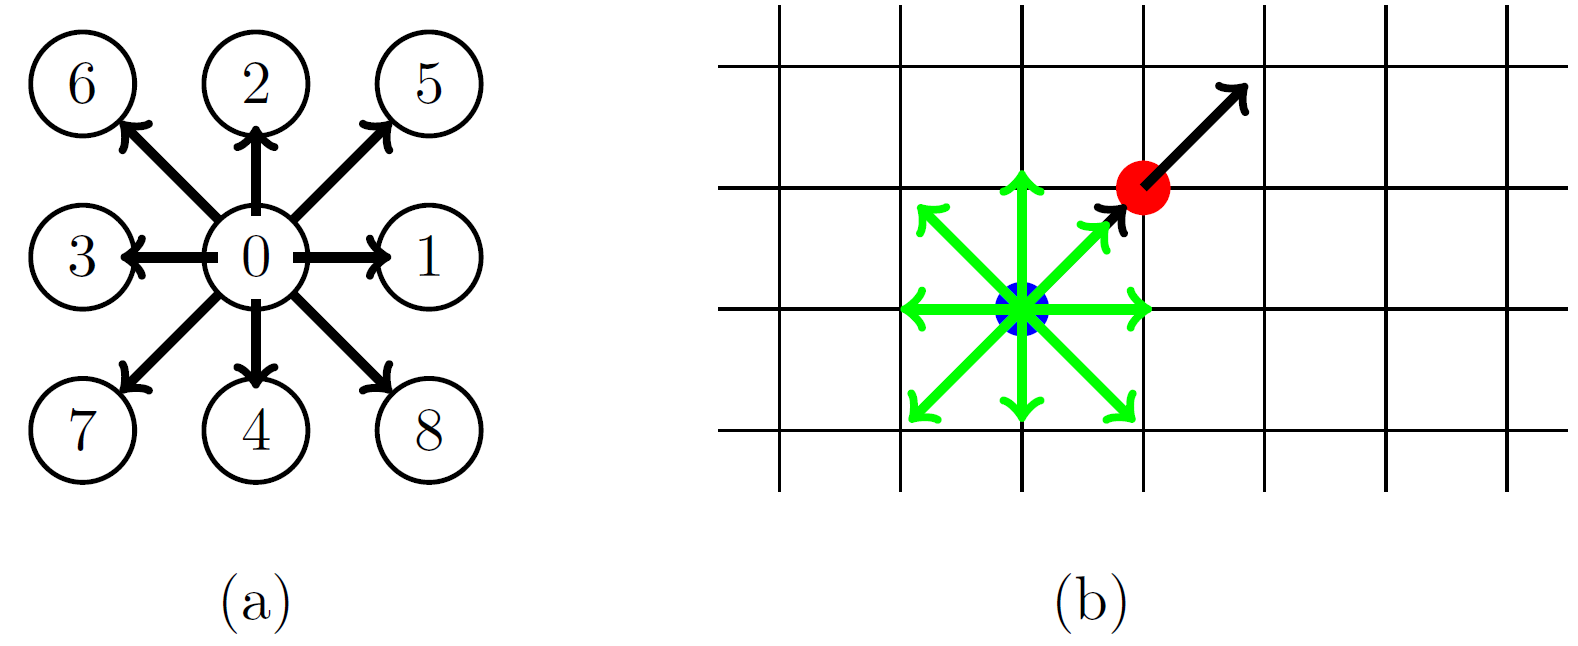
\includegraphics[width=10cm]{logos/Gitter_LBM.png}
        \caption{Visualization of the underlying grid including labled directions.}
        \label{fig:bte}
    \end{center}
\end{figure}

During the streaming, each particle moves in one of a set of predefined directions.
These particles can be further abstracted to densities, moving in specific directions.
The directions are given by the underlying grid and visualized in \ref{fig:bte}.
Each direction has a number in the interval [0, 8], e.g. direction 0 symbolizes not moving and density with the direction 1 moves to the rigth.
To allow moving further than to the closest neighbour, this streaming step is applied at each timestep (this is shown in part b) of \ref{fig:bte}).

\subsection{Collision}
Only applying streaming does not make sense, as long as particles cannot move through each other.
As this is not the case in this simulation, a collision between particles needs to be applied instantaneously with the streaming.

The effect of the collision is an exchange between the energy and momentum between 2 particles.
A collision is by nature probabilistic because 2 particles only collide by a certain chance.